% !TeX root = RJwrapper.tex
\title{corVis: An R Package for Visualising Associations and Conditional
Associations}
\author{by Amit Chinwan and Catherine Hurley}

\maketitle

\abstract{%
Correlation matrix displays are important tools to explore multivariate
datasets prior to modeling. These displays with other measures of
association can summarize interesting patterns to an analyst and assist
them in framing right questions while performing exploratory data
analysis. In this paper, we present new visualisation techniques to
visualise association between all the variable pairs in a dataset in a
single plot, which is something existing displays lack. We extend these
displays to regression and classification settings, where these could be
used to find out variables with high predictive power. Also, we propse
new methods to visualise trivariate relationship summaries using
conditioning. We use different layouts like: matrix or linear, to name a
few, for our displays which have their own advantages and disadvantages.
We use seriation in our displays which helps in highlighting interesting
patterns easily. The R package \emph{corVis} provides an implementation.
}

\hypertarget{introduction}{%
\section{Introduction}\label{introduction}}

Finding association among variables in a multivariate analysis is an
important step and can help an analyst to understand and frame right
questions about the data. In order to explore these relationships, the
analyst could use visual tools like correlation matrix plots (popularly
known as corrgrams \citep{friendly2002corrgrams}) to find out associated
variables. These displays are generally used with Pearson's correlation
coefficient and are therefore limited to only numeric features. In this
paper, we present new visualization techniques for displaying
association which will include different variable types, can compare
multiple measures of association and can conditionally visualize
association at different levels of a factor variable.

There have been extensions to corrgrams like:
\citep{buja2016visualization} and \citep{sCorrPlot}, which have been
proposed mainly for exploring correlations among the numeric variables
for a high dimensional dataset. We introduce a display which includes
all the variables of a dataset, irrespective of the data type, in a
conventional corrgram plot displaying every pairwise association. This
saves the effort and time of an analyst for exploring relationship among
all the variable pairs. \citep{kuhn2013applied} have proposed display
techniques to compare multiple association measures for every pair of
output variable and a predictor to measure the importance of each
predictor. This can help in summarizing a complex relationship more
efficiently as compared to using just one measure like Pearson's
correlation which can only find linear associations. In a similar way,
we propose different visualization techniques to compare multiple
association measures for all the variable pairs in a dataset which can
assist a user in finding interesting patterns.

\hypertarget{measures-of-association}{%
\section{Measures of Association}\label{measures-of-association}}

An association measure can be defined as a numerical summary quantifying
relationship between two or more variables. For example, Pearson's
correlation coefficient summarizes the strength and direction of the
linear relationship present between two \emph{numeric} variables and is
in the range \([-1,1]\). Similarly, distance correlation coefficient
measures the non-linear association between two \emph{numeric} variables
and summarizes it in \([0,1]\) where \(0\) suggests no non-linear
relationship and \(1\) suggests very high non-linear relationship. The
package provides a collection of various measures of association which
can be used to quantify the relationship between two variables and could
be used to explore patterns prior to modeling. The measures available in
the package are not limited to \emph{numeric} variables only and can be
used with \emph{categorical} and \emph{ordinal} variables as well.

\begin{itemize}
\item Pearson's correlation : Describe pearson's correlation.
\item Spearman's rank correlation.
\item Kendall's rank correlation.
\item Distance correlation.
\item Canonical correlations.
\item Maximal-information based non-parametric exploration (MINE) statistics.
\end{itemize}

\hypertarget{visualising-association}{%
\section{Visualising Association}\label{visualising-association}}

Correlation matrix plots (also called corrgrams) are popular tools for
exploring bivariate associations in multivariate datasets prior to
modelling. These displays are generally used with Pearson's correlation
coefficient and are thus suitable for numeric variables only. We propose
novel visualisations to display association for every variable pair in a
dataset in a single plot and show multiple bivariate measures of
association simultaneously to find out interesting patterns.

We propose a display for visualising association for different variable
types. This is an extension of existing corrgram which is only suitable
for numeric variables in a dataset. We calculate different assocaition
measures for different types of variable pairs and then plot them in a
similar way as it is done in a conventional corrgram. The traditional
method to find interesting bivariate relationships is to split the
dataset by the variable types and then analyse these one by one. Our
approach saves the effort and time of an analyst for exploring pairwise
relationships among all the variables in the dataset and can be done in
a single step.

We introduce a new structure for calculating association measures which
can be used to add other existing or new measures in the package. These
measures can then then be analysed and visualised using the plot
functions present in the package. For example, Cramer's V is a measure
to summarize association between two categorical variables using the
Chi-square test statistic. If a user wants to add Cramer's V to the
package, they can write a simple function and then can use it for their
analysis.

We consider matrix-type, linear and network-based layouts. A matrix-type
layout simplifies lookup, and different measures may be displayed on the
upper and lower diagonal. Linear layouts are more space-efficient than
matrix plots, but lookup is more challenging. Variable pairs can be
ordered by relevance (usually difference in measures of association or
across the factor levels), and less relevant pairs can be omitted.
Linear displays are also suitable to display associations between the
response and predictors only. Our selection criteria for a better
display were based on :

\begin{itemize}
\item Number of variables
\item Easier pixel-variable or variable-pixel
look up
\item Number of levels of a factor for conditional association displays
\end{itemize}

Figure \ref{fig:assoc-heatmap} shows this display for every variable
pair in the \emph{penguins} dataset from the \emph{palmerpenguins}
package. It shows a high positive Pearson's correlation among
flipper\_length\_mm and body\_mass\_g, flipper\_length\_mm and
bill\_length\_mm, and bill\_length\_mm and bodymass\_g. There seems to
be a strong negative Pearson's correlation between flipper\_length\_mm
and bill\_depth\_mm, and bill\_depth\_mm and body\_mass\_g. The plot
also shows that there is a high canonical correlation between species
and other variables except year and sex, and a high canonical
correlation between island and species, which traditional correlation
matrix display would omit as they are limited to numeric variable pairs
only. The variables in the display are ordered using average linkage
clustering method to find out highly associated variables quickly.

\begin{Schunk}
\begin{figure}

{\centering 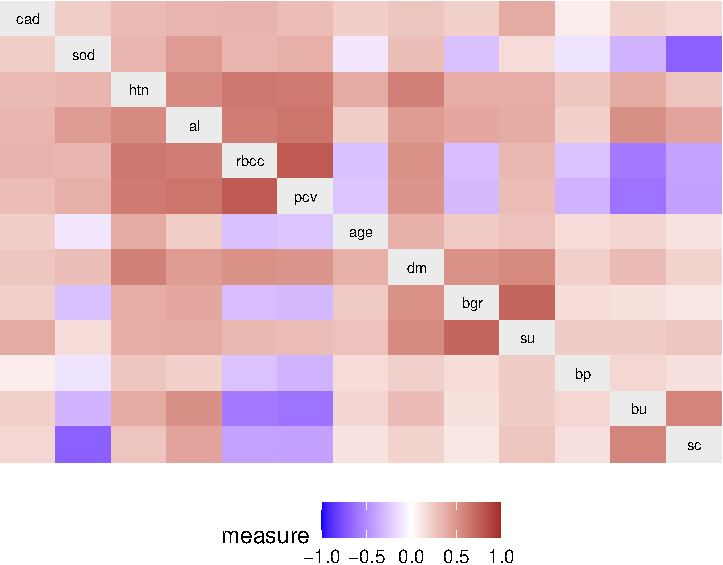
\includegraphics{rj_paper_files/figure-latex/assoc-heatmap-1} 

}

\caption[Association matrix display for penguins data]{Association matrix display for penguins data}\label{fig:assoc-heatmap}
\end{figure}
\end{Schunk}

We can also calculate multiple association measures for all the variable
pairs in the dataset and compare them. This will help in finding out
pairs of variables with a high difference among different measures and
one can investigate these bivariate relationships in more detail. The
\texttt{pairwise\_summary\_plot} function can be used to compare various
measures using the matrix layout. It plots multiple measures among the
variable pairs as bars, where each bar represents one measure of
association. Figure \ref{fig:compare-matrix} shows a matrix layout
comparing Pearson's and Spearman's correlation coefficient for the
numeric variable pairs in \emph{penguins} data.

\begin{Schunk}
\begin{figure}

{\centering 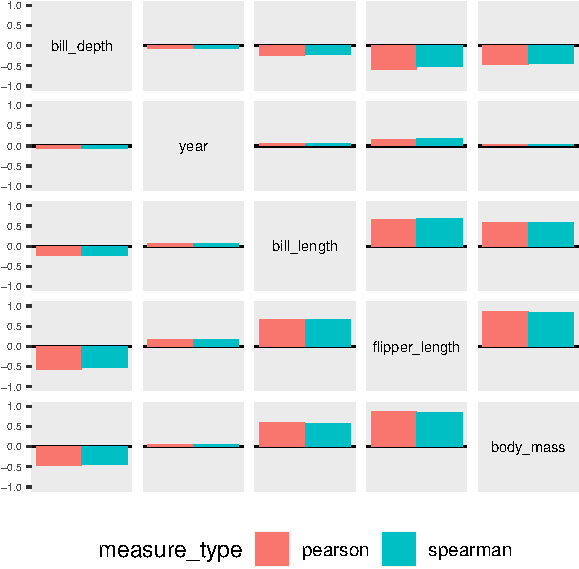
\includegraphics{rj_paper_files/figure-latex/compare-matrix-1} 

}

\caption[Comparing Pearson's and Spearman's correlation coefficient]{Comparing Pearson's and Spearman's correlation coefficient}\label{fig:compare-matrix}
\end{figure}
\end{Schunk}

In addition to matrix layout, we can also use linear layouts for
comparing multiple measures. Figure \ref{fig:compare-linear} shows a
linear layout comparing multiple association measures for all the
variable pairs in the penguins data. Linear layouts seems to be more
suitable when comparing high number of association measures.

\begin{Schunk}
\begin{figure}

{\centering 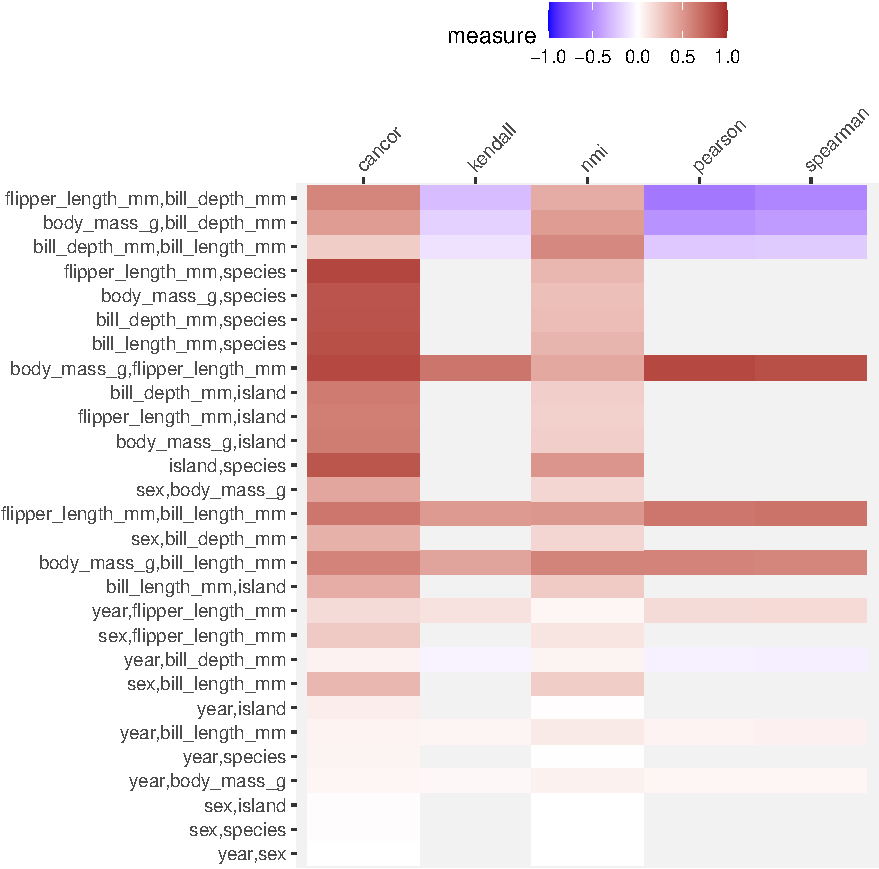
\includegraphics{rj_paper_files/figure-latex/compare-linear-1} 

}

\caption[Comparing multiple association measures using a linear layout]{Comparing multiple association measures using a linear layout}\label{fig:compare-linear}
\end{figure}
\end{Schunk}

\hypertarget{visualising-conditional-association}{%
\section{Visualising Conditional
Association}\label{visualising-conditional-association}}

The package includes a function \texttt{calc\_assoc\_by} which
calculates the pairwise association at different levels of a categorical
conditioning variable. This helps in finding out interesting variable
triples which can be explored further prior to modeling. Figure
\ref{fig:cond-assoc} shows a conditional association plot for the
\emph{penguins} data. Each cell corresponding to a variable pair shows
three bars which correspond to the association measure (Pearson's
correlation for numeric pair and Normalized mutual information for other
combination of variables) calculated at the levels of conditioning
variable \emph{island}. The dashed line represents the overall
association measure. The plot shows that there is a high value for
normalised mutual information between bill\_length\_mm and species for
the penguins which lived in \emph{Biscoe} island compared to the
penguins which lived in \emph{Dream} island. It can also be seen that
the cell corresponding to variable pair flipper\_length\_mm and
bill\_depth\_mm has a high negative overall Pearson's correlation and
for the penguins which lived in \emph{Biscoe} island but positive
correlation for penguins which lived in \emph{Dream} and
\emph{Torgersen} island. This is an instance of Simpson's paradox which
can be taken into account during the modeling step.

\begin{Schunk}
\begin{figure}

{\centering 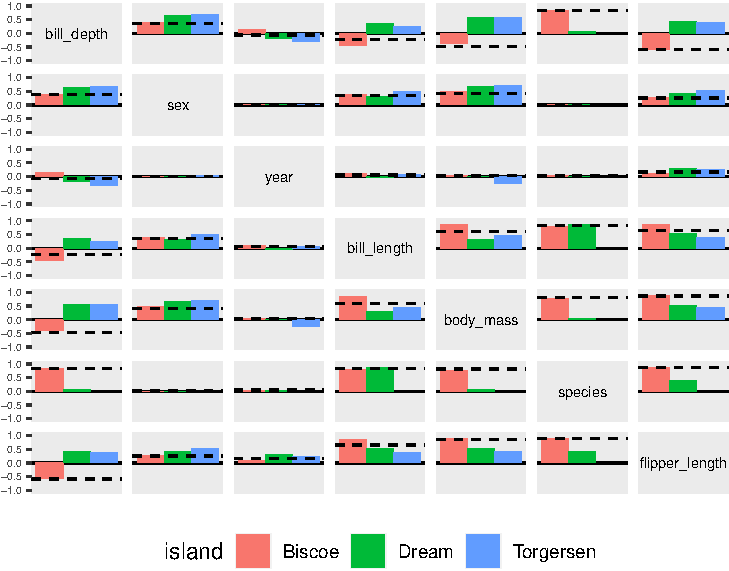
\includegraphics{rj_paper_files/figure-latex/cond-assoc-1} 

}

\caption[Figure 4]{Figure 4: Conditional Association plot}\label{fig:cond-assoc}
\end{figure}
\end{Schunk}

\hypertarget{discussion}{%
\section{Discussion}\label{discussion}}

We have displayed various tooltips that are available in the package
\pkg{ToOoOlTiPs}.

\bibliography{RJreferences.bib}

\address{%
Amit Chinwan\\
Maynooth University\\%
Hamilton Institute\\ Maynooth, Ireland\\
%
%
%
\href{mailto:amit.chinwan.2019@mumail.ie}{\nolinkurl{amit.chinwan.2019@mumail.ie}}%
}

\address{%
Catherine Hurley\\
Maynooth University\\%
Department of Mathematics and Statistics\\ Maynooth, Ireland\\
%
%
%
\href{mailto:catherine.hurley@mu.ie}{\nolinkurl{catherine.hurley@mu.ie}}%
}
